% Supplementary material for the HyperShield benchmark paper.
% Build: python make_supplement.py (from the repository root), then in this folder
%        pdflatex Supplementary_Material.tex  (run twice).
\documentclass[11pt,a4paper]{article}
\usepackage[T1]{fontenc}
\usepackage{lmodern}
\usepackage{mathptmx}
\usepackage[margin=2cm]{geometry}
\usepackage{amsmath}
\usepackage{booktabs}
\usepackage{array}
\usepackage{graphicx}
\usepackage{caption}
\usepackage{enumitem}
\usepackage{xurl}
\usepackage{placeins}
\usepackage[hidelinks]{hyperref}

\captionsetup{font=small,labelfont=bf,labelsep=period}
\renewcommand{\thetable}{S\arabic{table}}
\renewcommand{\thefigure}{S\arabic{figure}}
\setlength{\parskip}{4pt}
\setlength{\parindent}{0pt}

\newcommand{\repo}{\url{https://github.com/labibibnmuzahid/hypershield-benchmark}}

\begin{document}

\begin{center}
{\Large\bfseries Supplementary material}\\[6pt]
{\large Uncertainty-aware space--ground sensor fusion for tracking maneuvering hypersonic targets: A reproducible simulation benchmark}\\[10pt]
Abdullah Al Junayed$^{a,*}$, Labib Ibn Muzahid$^{b}$\\[4pt]
{\small $^a$Department of Mechanical Engineering and $^b$Department of Computer Science and Engineering,\\
International University of Business Agriculture and Technology (IUBAT), Dhaka 1230, Bangladesh\\
$^*$Corresponding author: junayed.mahin@iubat.education}
\end{center}

\section*{S1. Contents}

This supplement extends the results reported in the paper. Section and table numbers without the prefix S refer to the paper.

\begin{itemize}[leftmargin=*,itemsep=1pt]
\item Tables S1--S3: every sensing configuration and estimator at each maneuver level, with all metrics and confidence intervals (Section 7.2 and Table 5 report the medium level).
\item Table S4: all 36 paired estimator comparisons; Table S5: all 24 paired comparisons of fused against single-sensor tracking (Sections 7.2--7.3; Table 6 reports the fused subset).
\item Tables S6--S7: credibility diagnostics of the stated covariance for every estimator (Section 7.4).
\item Tables S8--S9: every value of the sensitivity sweeps for all four estimators (Section 7.5 and Fig.~9).
\item Table S10: the complete process-noise tuning grid (Appendix A and Table A.1); Table S11: statistics of the held-out scenarios (Section 4); Table S12: computational cost of every cell (Section 7.6).
\item Figure S1: mean OSPA and track availability over time; Figure S2: distributions of the paired per-run OSPA differences behind Table 6.
\item Section S7: implementation choices where the paper leaves a detail open; Table S13: the 31 automated verification tests; Section S9: how to reproduce every number.
\end{itemize}

Every value in this supplement is generated by \texttt{make\_supplement.py} from the released result files; none was entered by hand. The same tables are provided as CSV files (Supplementary data, \texttt{Supplementary\_Data.zip}, and \texttt{results/supplement/} in the repository). The code, configurations, seeds and results are openly available at \repo.

\section*{S2. Results for every configuration and estimator}

Tables S1--S3 list all 36 cells of the main evaluation (3 sensing configurations $\times$ 4 estimators $\times$ 3 maneuver levels, 500 held-out runs per maneuver level). Figure S1 shows how the advantage of fusion builds up over the 480 s scenario: the IR layer provides a track within seconds, the radar contributes only after the target enters its coverage, and the fused tracker keeps the lowest OSPA throughout.

\begin{table}[!htbp]
\caption{All sensing configurations and estimators at the low (0.5 g) maneuver level (500 held-out runs each).}
\label{tab:S1}
\centering\footnotesize\setlength{\tabcolsep}{3.5pt}
\begin{tabular}{@{}lcccccccccc@{}}
\toprule
Estimator & OSPA (km) & Custody & Contin. & Segments & TTFT & Ever & RMSE & ANEES & $C_{50}$ & $C_{95}$ \\
 & [95\% CI] & (\%) & (\%) & per run & (s) & tracked (\%) & (km) & [95\% CI] & & \\
\midrule
\multicolumn{11}{@{}l}{\textit{IR only}} \\
EKF-CV & 2.13 [2.02, 2.23] & 77.4 & 83.6 & 3.84 & 4 & 100.0 & 3.59 & 2.86 [2.66, 3.08] & 0.578 & 0.924 \\
UKF-CV & 2.13 [2.02, 2.23] & 77.3 & 83.5 & 3.85 & 4 & 100.0 & 3.60 & 2.86 [2.66, 3.08] & 0.577 & 0.924 \\
EKF-CA & 2.27 [2.15, 2.37] & 74.6 & 83.3 & 4.29 & 4 & 100.0 & 4.40 & 3.03 [2.83, 3.23] & 0.522 & 0.899 \\
IMM-CV/CA & 2.05 [1.94, 2.16] & 78.6 & 83.9 & 3.76 & 4 & 100.0 & 3.49 & 2.40 [2.24, 2.57] & 0.525 & 0.918 \\
\midrule
\multicolumn{11}{@{}l}{\textit{Radar only}} \\
EKF-CV & 6.37 [6.25, 6.49] & 36.7 & 38.0 & 1.35 & 285 & 99.4 & 0.61 & 2.29 [1.96, 2.67] & 0.558 & 0.958 \\
UKF-CV & 6.37 [6.25, 6.49] & 36.7 & 38.0 & 1.36 & 285 & 99.4 & 0.61 & 2.17 [1.87, 2.51] & 0.558 & 0.958 \\
EKF-CA & 6.38 [6.26, 6.50] & 36.1 & 38.1 & 1.48 & 283.5 & 99.4 & 0.66 & 2.37 [2.09, 2.69] & 0.533 & 0.951 \\
IMM-CV/CA & 6.35 [6.23, 6.48] & 36.9 & 38.1 & 1.35 & 284 & 99.4 & 0.59 & 2.27 [1.99, 2.59] & 0.516 & 0.946 \\
\midrule
\multicolumn{11}{@{}l}{\textit{Fused}} \\
EKF-CV & 1.46 [1.38, 1.55] & 85.1 & 89.3 & 3.05 & 4 & 100.0 & 2.94 & 2.31 [2.15, 2.48] & 0.570 & 0.938 \\
UKF-CV & 1.46 [1.38, 1.55] & 85.1 & 89.3 & 3.06 & 4 & 100.0 & 2.94 & 2.29 [2.14, 2.46] & 0.570 & 0.938 \\
EKF-CA & 1.56 [1.47, 1.64] & 83.2 & 89.1 & 3.37 & 4 & 100.0 & 3.66 & 2.39 [2.24, 2.55] & 0.525 & 0.919 \\
IMM-CV/CA & 1.40 [1.32, 1.49] & 85.9 & 89.6 & 3.00 & 4 & 100.0 & 2.88 & 2.01 [1.89, 2.14] & 0.520 & 0.929 \\
\bottomrule
\end{tabular}

\smallskip
\parbox{\textwidth}{\footnotesize OSPA: mean OSPA distance, cut-off 10 km. Custody: share of epochs with a confirmed track within 1 km. Contin.: share of epochs with a confirmed track. Segments: confirmed track segments per run. TTFT: median time to first track within 5 km (runs never tracked count as infinite; a median over an even number of runs can end in .5, which the paper rounds to whole seconds). Ever tracked: share of runs with at least one such track. RMSE: over epochs with a track. ANEES: normalized (ideal 1). $C_\alpha$: empirical coverage of the nominal $\alpha$ ellipsoid. Confidence intervals: run-level percentile bootstrap, 2000 resamples.}
\end{table}

\begin{table}[!htbp]
\caption{All sensing configurations and estimators at the medium (2 g) maneuver level (500 held-out runs each).}
\label{tab:S2}
\centering\footnotesize\setlength{\tabcolsep}{3.5pt}
\begin{tabular}{@{}lcccccccccc@{}}
\toprule
Estimator & OSPA (km) & Custody & Contin. & Segments & TTFT & Ever & RMSE & ANEES & $C_{50}$ & $C_{95}$ \\
 & [95\% CI] & (\%) & (\%) & per run & (s) & tracked (\%) & (km) & [95\% CI] & & \\
\midrule
\multicolumn{11}{@{}l}{\textit{IR only}} \\
EKF-CV & 2.21 [2.10, 2.32] & 75.5 & 83.2 & 3.94 & 4 & 100.0 & 4.02 & 3.18 [2.94, 3.43] & 0.547 & 0.916 \\
UKF-CV & 2.20 [2.09, 2.32] & 75.5 & 83.2 & 3.94 & 4 & 100.0 & 4.02 & 3.15 [2.92, 3.39] & 0.547 & 0.916 \\
EKF-CA & 2.32 [2.21, 2.44] & 73.6 & 83.0 & 4.37 & 4 & 100.0 & 4.74 & 3.22 [3.01, 3.46] & 0.508 & 0.891 \\
IMM-CV/CA & 2.13 [2.02, 2.24] & 76.7 & 83.6 & 3.81 & 4 & 100.0 & 4.00 & 2.61 [2.45, 2.77] & 0.476 & 0.894 \\
\midrule
\multicolumn{11}{@{}l}{\textit{Radar only}} \\
EKF-CV & 6.48 [6.36, 6.60] & 35.3 & 36.9 & 1.40 & 293.5 & 98.8 & 0.66 & 2.66 [2.30, 3.09] & 0.532 & 0.950 \\
UKF-CV & 6.48 [6.37, 6.60] & 35.3 & 36.9 & 1.39 & 293.5 & 98.8 & 0.66 & 2.48 [2.15, 2.87] & 0.532 & 0.950 \\
EKF-CA & 6.48 [6.37, 6.60] & 34.8 & 37.0 & 1.50 & 293 & 98.8 & 0.70 & 2.45 [2.15, 2.78] & 0.524 & 0.945 \\
IMM-CV/CA & 6.48 [6.36, 6.59] & 35.3 & 37.0 & 1.40 & 293.5 & 98.8 & 0.66 & 2.48 [2.17, 2.84] & 0.474 & 0.927 \\
\midrule
\multicolumn{11}{@{}l}{\textit{Fused}} \\
EKF-CV & 1.56 [1.48, 1.65] & 83.4 & 88.6 & 3.15 & 4 & 100.0 & 3.19 & 2.58 [2.39, 2.79] & 0.546 & 0.930 \\
UKF-CV & 1.56 [1.48, 1.64] & 83.5 & 88.6 & 3.15 & 4 & 100.0 & 3.18 & 2.56 [2.36, 2.76] & 0.546 & 0.931 \\
EKF-CA & 1.64 [1.56, 1.73] & 82.2 & 88.4 & 3.49 & 4 & 100.0 & 3.70 & 2.64 [2.46, 2.83] & 0.515 & 0.913 \\
IMM-CV/CA & 1.51 [1.43, 1.59] & 84.1 & 88.9 & 3.07 & 4 & 100.0 & 3.23 & 2.30 [2.16, 2.46] & 0.477 & 0.905 \\
\bottomrule
\end{tabular}

\smallskip
\parbox{\textwidth}{\footnotesize OSPA: mean OSPA distance, cut-off 10 km. Custody: share of epochs with a confirmed track within 1 km. Contin.: share of epochs with a confirmed track. Segments: confirmed track segments per run. TTFT: median time to first track within 5 km (runs never tracked count as infinite; a median over an even number of runs can end in .5, which the paper rounds to whole seconds). Ever tracked: share of runs with at least one such track. RMSE: over epochs with a track. ANEES: normalized (ideal 1). $C_\alpha$: empirical coverage of the nominal $\alpha$ ellipsoid. Confidence intervals: run-level percentile bootstrap, 2000 resamples.}
\end{table}

\begin{table}[!htbp]
\caption{All sensing configurations and estimators at the high (4 g) maneuver level (500 held-out runs each).}
\label{tab:S3}
\centering\footnotesize\setlength{\tabcolsep}{3.5pt}
\begin{tabular}{@{}lcccccccccc@{}}
\toprule
Estimator & OSPA (km) & Custody & Contin. & Segments & TTFT & Ever & RMSE & ANEES & $C_{50}$ & $C_{95}$ \\
 & [95\% CI] & (\%) & (\%) & per run & (s) & tracked (\%) & (km) & [95\% CI] & & \\
\midrule
\multicolumn{11}{@{}l}{\textit{IR only}} \\
EKF-CV & 2.29 [2.18, 2.40] & 73.8 & 83.6 & 4.13 & 4 & 100.0 & 4.14 & 3.81 [3.54, 4.07] & 0.468 & 0.871 \\
UKF-CV & 2.29 [2.17, 2.40] & 73.8 & 83.6 & 4.13 & 4 & 100.0 & 4.12 & 3.79 [3.53, 4.06] & 0.468 & 0.871 \\
EKF-CA & 2.33 [2.22, 2.44] & 73.1 & 83.5 & 4.42 & 4 & 100.0 & 4.75 & 3.62 [3.41, 3.86] & 0.466 & 0.861 \\
IMM-CV/CA & 2.23 [2.12, 2.34] & 74.6 & 83.8 & 4.07 & 4 & 100.0 & 4.14 & 3.40 [3.19, 3.62] & 0.430 & 0.848 \\
\midrule
\multicolumn{11}{@{}l}{\textit{Radar only}} \\
EKF-CV & 6.69 [6.56, 6.83] & 32.4 & 34.9 & 1.37 & 300.5 & 96.4 & 0.69 & 2.41 [2.06, 2.77] & 0.469 & 0.921 \\
UKF-CV & 6.69 [6.56, 6.83] & 32.5 & 34.9 & 1.37 & 300.5 & 96.4 & 0.69 & 2.25 [1.93, 2.59] & 0.470 & 0.921 \\
EKF-CA & 6.68 [6.55, 6.82] & 32.5 & 35.0 & 1.46 & 300 & 96.6 & 0.72 & 2.24 [1.97, 2.52] & 0.494 & 0.935 \\
IMM-CV/CA & 6.68 [6.55, 6.82] & 32.7 & 34.9 & 1.38 & 300.5 & 96.4 & 0.68 & 2.26 [1.98, 2.56] & 0.451 & 0.910 \\
\midrule
\multicolumn{11}{@{}l}{\textit{Fused}} \\
EKF-CV & 1.62 [1.53, 1.70] & 82.1 & 88.9 & 3.36 & 4 & 100.0 & 3.29 & 3.05 [2.83, 3.27] & 0.481 & 0.895 \\
UKF-CV & 1.62 [1.53, 1.70] & 82.2 & 88.9 & 3.36 & 4 & 100.0 & 3.28 & 3.02 [2.81, 3.24] & 0.481 & 0.896 \\
EKF-CA & 1.65 [1.56, 1.73] & 81.6 & 88.9 & 3.62 & 4 & 100.0 & 3.80 & 2.92 [2.74, 3.12] & 0.476 & 0.886 \\
IMM-CV/CA & 1.57 [1.49, 1.66] & 82.7 & 89.1 & 3.34 & 4 & 100.0 & 3.33 & 2.84 [2.67, 3.04] & 0.440 & 0.872 \\
\bottomrule
\end{tabular}

\smallskip
\parbox{\textwidth}{\footnotesize OSPA: mean OSPA distance, cut-off 10 km. Custody: share of epochs with a confirmed track within 1 km. Contin.: share of epochs with a confirmed track. Segments: confirmed track segments per run. TTFT: median time to first track within 5 km (runs never tracked count as infinite; a median over an even number of runs can end in .5, which the paper rounds to whole seconds). Ever tracked: share of runs with at least one such track. RMSE: over epochs with a track. ANEES: normalized (ideal 1). $C_\alpha$: empirical coverage of the nominal $\alpha$ ellipsoid. Confidence intervals: run-level percentile bootstrap, 2000 resamples.}
\end{table}


\begin{figure}[!htbp]
\centering
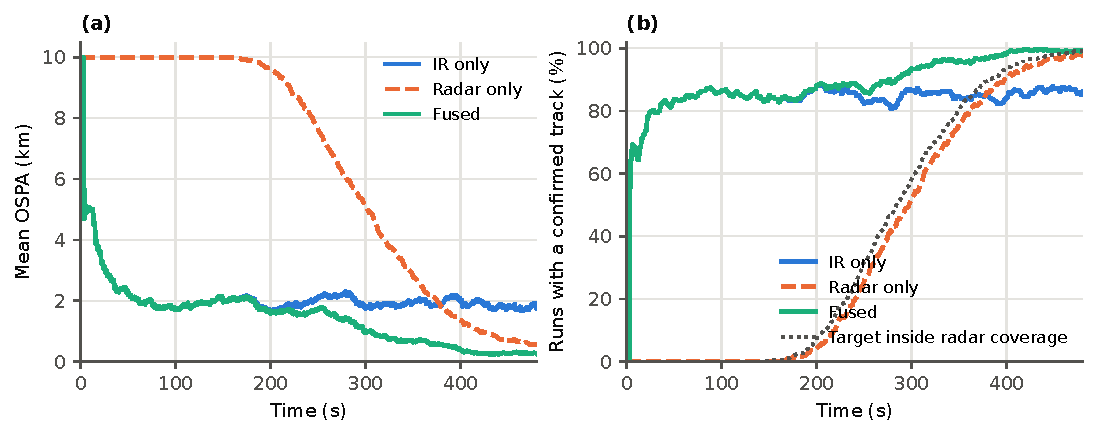
\includegraphics[width=\textwidth]{Figure_S1.pdf}
\caption{Accuracy and track availability over time, IMM-CV/CA at the medium maneuver level (500 runs). (a) Mean OSPA at each epoch (cut-off 10 km). (b) Share of runs holding a confirmed track; the dotted line is the share of runs whose target is inside radar coverage.}
\label{fig:S1}
\end{figure}

\FloatBarrier
\section*{S3. Paired comparisons}

Table S4 lists every estimator comparison in the Holm family used in the paper, and Table S5 every comparison of fused against single-sensor tracking. Figure S2 shows the run-level distributions behind the ``Better'' column of Table 6 for the IMM against EKF-CV: most differences are small and negative, which is why a 3--4\% mean improvement is highly significant in the paired test.

\begin{table}[!htbp]
\caption{All 36 paired estimator comparisons of per-run OSPA (one Holm family).}
\label{tab:S4}
\centering\footnotesize\setlength{\tabcolsep}{4pt}
\begin{tabular}{@{}lllrrrrr@{}}
\toprule
Maneuver & Sensing & Comparison & $\Delta$ OSPA (km) & $\Delta$ (\%) & Better (\%) & $p$ & Holm $p$ \\
\midrule
Low & IR only & IMM-CV/CA vs EKF-CV & $-0.0794$ & $-3.73$ & 80.6 & $1.8\times10^{-32}$ & $5.0\times10^{-31}$ \\
Low & IR only & IMM-CV/CA vs UKF-CV & $-0.0821$ & $-3.85$ & 81.0 & $1.1\times10^{-33}$ & $3.3\times10^{-32}$ \\
Low & IR only & IMM-CV/CA vs EKF-CA & $-0.2162$ & $-9.54$ & 86.6 & $2.0\times10^{-44}$ & $6.8\times10^{-43}$ \\
Low & IR only & UKF-CV vs EKF-CV & $+0.0028$ & $+0.13$ & 54.2 & 0.007 & 0.037 \\
\addlinespace[2pt]
Low & Radar only & IMM-CV/CA vs EKF-CV & $-0.0160$ & $-0.25$ & 71.8 & $1.5\times10^{-29}$ & $3.9\times10^{-28}$ \\
Low & Radar only & IMM-CV/CA vs UKF-CV & $-0.0162$ & $-0.25$ & 71.6 & $4.5\times10^{-29}$ & $1.2\times10^{-27}$ \\
Low & Radar only & IMM-CV/CA vs EKF-CA & $-0.0241$ & $-0.38$ & 86.2 & $1.2\times10^{-46}$ & $4.2\times10^{-45}$ \\
Low & Radar only & UKF-CV vs EKF-CV & $+0.0002$ & $+0.00$ & 36.6 & $5.8\times10^{-11}$ & $9.2\times10^{-10}$ \\
\addlinespace[2pt]
Low & Fused & IMM-CV/CA vs EKF-CV & $-0.0568$ & $-3.89$ & 83.0 & $5.6\times10^{-33}$ & $1.7\times10^{-31}$ \\
Low & Fused & IMM-CV/CA vs UKF-CV & $-0.0560$ & $-3.83$ & 83.4 & $6.9\times10^{-34}$ & $2.2\times10^{-32}$ \\
Low & Fused & IMM-CV/CA vs EKF-CA & $-0.1508$ & $-9.70$ & 85.8 & $1.7\times10^{-40}$ & $5.9\times10^{-39}$ \\
Low & Fused & UKF-CV vs EKF-CV & $-0.0008$ & $-0.05$ & 52.4 & 0.008 & 0.037 \\
\addlinespace[2pt]
\midrule
Medium & IR only & IMM-CV/CA vs EKF-CV & $-0.0795$ & $-3.60$ & 77.6 & $4.4\times10^{-25}$ & $1.1\times10^{-23}$ \\
Medium & IR only & IMM-CV/CA vs UKF-CV & $-0.0770$ & $-3.49$ & 77.4 & $2.1\times10^{-24}$ & $5.0\times10^{-23}$ \\
Medium & IR only & IMM-CV/CA vs EKF-CA & $-0.1971$ & $-8.48$ & 79.4 & $3.4\times10^{-35}$ & $1.1\times10^{-33}$ \\
Medium & IR only & UKF-CV vs EKF-CV & $-0.0024$ & $-0.11$ & 56.4 & $1.2\times10^{-5}$ & $9.7\times10^{-5}$ \\
\addlinespace[2pt]
Medium & Radar only & IMM-CV/CA vs EKF-CV & $-0.0034$ & $-0.05$ & 53.2 & 0.016 & 0.047 \\
Medium & Radar only & IMM-CV/CA vs UKF-CV & $-0.0054$ & $-0.08$ & 53.2 & 0.020 & 0.047 \\
Medium & Radar only & IMM-CV/CA vs EKF-CA & $-0.0081$ & $-0.12$ & 72.6 & $2.7\times10^{-21}$ & $5.6\times10^{-20}$ \\
Medium & Radar only & UKF-CV vs EKF-CV & $+0.0021$ & $+0.03$ & 33.8 & $4.2\times10^{-15}$ & $7.1\times10^{-14}$ \\
\addlinespace[2pt]
Medium & Fused & IMM-CV/CA vs EKF-CV & $-0.0537$ & $-3.43$ & 76.0 & $5.6\times10^{-23}$ & $1.3\times10^{-21}$ \\
Medium & Fused & IMM-CV/CA vs UKF-CV & $-0.0510$ & $-3.26$ & 75.8 & $1.4\times10^{-22}$ & $3.2\times10^{-21}$ \\
Medium & Fused & IMM-CV/CA vs EKF-CA & $-0.1316$ & $-8.01$ & 78.6 & $9.7\times10^{-33}$ & $2.8\times10^{-31}$ \\
Medium & Fused & UKF-CV vs EKF-CV & $-0.0027$ & $-0.17$ & 56.2 & $2.9\times10^{-5}$ & $2.1\times10^{-4}$ \\
\addlinespace[2pt]
\midrule
High & IR only & IMM-CV/CA vs EKF-CV & $-0.0602$ & $-2.63$ & 68.4 & $3.9\times10^{-9}$ & $4.7\times10^{-8}$ \\
High & IR only & IMM-CV/CA vs UKF-CV & $-0.0554$ & $-2.42$ & 67.8 & $2.6\times10^{-8}$ & $2.9\times10^{-7}$ \\
High & IR only & IMM-CV/CA vs EKF-CA & $-0.1022$ & $-4.38$ & 65.0 & $4.1\times10^{-10}$ & $5.8\times10^{-9}$ \\
High & IR only & UKF-CV vs EKF-CV & $-0.0048$ & $-0.21$ & 54.2 & 0.004 & 0.021 \\
\addlinespace[2pt]
High & Radar only & IMM-CV/CA vs EKF-CV & $-0.0122$ & $-0.18$ & 65.8 & $3.4\times10^{-20}$ & $6.8\times10^{-19}$ \\
High & Radar only & IMM-CV/CA vs UKF-CV & $-0.0086$ & $-0.13$ & 65.6 & $2.7\times10^{-19}$ & $5.1\times10^{-18}$ \\
High & Radar only & IMM-CV/CA vs EKF-CA & $+0.0027$ & $+0.04$ & 61.2 & $7.1\times10^{-6}$ & $6.4\times10^{-5}$ \\
High & Radar only & UKF-CV vs EKF-CV & $-0.0036$ & $-0.05$ & 33.0 & $2.2\times10^{-15}$ & $4.0\times10^{-14}$ \\
\addlinespace[2pt]
High & Fused & IMM-CV/CA vs EKF-CV & $-0.0471$ & $-2.90$ & 69.6 & $1.2\times10^{-10}$ & $1.7\times10^{-9}$ \\
High & Fused & IMM-CV/CA vs UKF-CV & $-0.0430$ & $-2.66$ & 69.2 & $1.2\times10^{-9}$ & $1.5\times10^{-8}$ \\
High & Fused & IMM-CV/CA vs EKF-CA & $-0.0745$ & $-4.52$ & 62.2 & $6.5\times10^{-8}$ & $6.5\times10^{-7}$ \\
High & Fused & UKF-CV vs EKF-CV & $-0.0041$ & $-0.25$ & 54.6 & 0.061 & 0.061 \\
\addlinespace[2pt]
\bottomrule
\end{tabular}

\smallskip
\parbox{\textwidth}{\footnotesize $\Delta$: mean per-run OSPA difference, first minus second estimator; $\Delta$ (\%): relative to the second estimator. Better: share of runs in which the first estimator had the lower OSPA. $p$: two-sided Wilcoxon signed-rank test on 500 paired runs; Holm $p$: adjusted over all 36 comparisons.}
\end{table}

\begin{table}[!htbp]
\caption{All 24 paired comparisons of fused against single-sensor tracking (per-run OSPA, one Holm family).}
\label{tab:S5}
\centering\footnotesize\setlength{\tabcolsep}{4pt}
\begin{tabular}{@{}lllrrrrr@{}}
\toprule
Maneuver & Estimator & Comparison & $\Delta$ OSPA (km) & $\Delta$ (\%) & Better (\%) & $p$ & Holm $p$ \\
\midrule
Low & EKF-CV & Fused vs IR only & $-0.667$ & $-31.3$ & 97.8 & $1.2\times10^{-79}$ & $1.3\times10^{-78}$ \\
Low & EKF-CV & Fused vs Radar only & $-4.905$ & $-77.0$ & 100.0 & $1.3\times10^{-83}$ & $3.0\times10^{-82}$ \\
Low & UKF-CV & Fused vs IR only & $-0.670$ & $-31.4$ & 97.8 & $1.2\times10^{-79}$ & $1.3\times10^{-78}$ \\
Low & UKF-CV & Fused vs Radar only & $-4.906$ & $-77.1$ & 100.0 & $1.3\times10^{-83}$ & $3.0\times10^{-82}$ \\
Low & EKF-CA & Fused vs IR only & $-0.709$ & $-31.3$ & 98.0 & $1.1\times10^{-80}$ & $1.3\times10^{-79}$ \\
Low & EKF-CA & Fused vs Radar only & $-4.819$ & $-75.6$ & 100.0 & $1.3\times10^{-83}$ & $3.0\times10^{-82}$ \\
Low & IMM-CV/CA & Fused vs IR only & $-0.644$ & $-31.4$ & 97.4 & $5.3\times10^{-79}$ & $4.7\times10^{-78}$ \\
Low & IMM-CV/CA & Fused vs Radar only & $-4.946$ & $-77.9$ & 100.0 & $1.3\times10^{-83}$ & $3.0\times10^{-82}$ \\
\midrule
Medium & EKF-CV & Fused vs IR only & $-0.642$ & $-29.1$ & 97.0 & $2.0\times10^{-78}$ & $1.6\times10^{-77}$ \\
Medium & EKF-CV & Fused vs Radar only & $-4.915$ & $-75.8$ & 100.0 & $1.3\times10^{-83}$ & $3.0\times10^{-82}$ \\
Medium & UKF-CV & Fused vs IR only & $-0.642$ & $-29.1$ & 97.0 & $2.2\times10^{-78}$ & $1.6\times10^{-77}$ \\
Medium & UKF-CV & Fused vs Radar only & $-4.920$ & $-75.9$ & 100.0 & $1.3\times10^{-83}$ & $3.0\times10^{-82}$ \\
Medium & EKF-CA & Fused vs IR only & $-0.681$ & $-29.3$ & 97.0 & $2.3\times10^{-78}$ & $1.6\times10^{-77}$ \\
Medium & EKF-CA & Fused vs Radar only & $-4.842$ & $-74.7$ & 100.0 & $1.3\times10^{-83}$ & $3.0\times10^{-82}$ \\
Medium & IMM-CV/CA & Fused vs IR only & $-0.616$ & $-29.0$ & 96.8 & $3.0\times10^{-77}$ & $6.1\times10^{-77}$ \\
Medium & IMM-CV/CA & Fused vs Radar only & $-4.965$ & $-76.7$ & 100.0 & $1.3\times10^{-83}$ & $3.0\times10^{-82}$ \\
\midrule
High & EKF-CV & Fused vs IR only & $-0.668$ & $-29.2$ & 95.6 & $5.7\times10^{-78}$ & $2.3\times10^{-77}$ \\
High & EKF-CV & Fused vs Radar only & $-5.072$ & $-75.8$ & 100.0 & $1.3\times10^{-83}$ & $3.0\times10^{-82}$ \\
High & UKF-CV & Fused vs IR only & $-0.668$ & $-29.2$ & 95.6 & $5.7\times10^{-78}$ & $2.3\times10^{-77}$ \\
High & UKF-CV & Fused vs Radar only & $-5.073$ & $-75.8$ & 100.0 & $1.3\times10^{-83}$ & $3.0\times10^{-82}$ \\
High & EKF-CA & Fused vs IR only & $-0.683$ & $-29.3$ & 95.2 & $2.0\times10^{-78}$ & $1.6\times10^{-77}$ \\
High & EKF-CA & Fused vs Radar only & $-5.030$ & $-75.3$ & 100.0 & $1.3\times10^{-83}$ & $3.0\times10^{-82}$ \\
High & IMM-CV/CA & Fused vs IR only & $-0.655$ & $-29.4$ & 94.8 & $8.3\times10^{-77}$ & $8.3\times10^{-77}$ \\
High & IMM-CV/CA & Fused vs Radar only & $-5.107$ & $-76.4$ & 100.0 & $1.3\times10^{-83}$ & $3.0\times10^{-82}$ \\
\bottomrule
\end{tabular}

\smallskip
\parbox{\textwidth}{\footnotesize $\Delta$: mean per-run OSPA difference, fused minus single-sensor; $\Delta$ (\%): relative to the single-sensor value. Better: share of runs in which fused tracking had the lower OSPA. $p$: two-sided Wilcoxon signed-rank test; Holm $p$: adjusted over the 24 comparisons.}
\end{table}


\begin{figure}[!htbp]
\centering
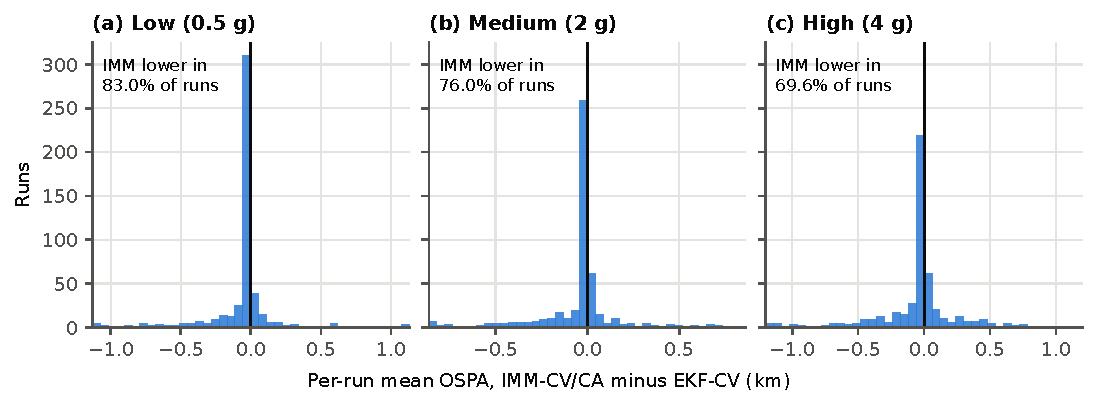
\includegraphics[width=\textwidth]{Figure_S2.pdf}
\caption{Distribution of the per-run OSPA difference between IMM-CV/CA and EKF-CV in the fused configuration (500 paired runs per maneuver level). Negative values favor the IMM. Differences beyond the 99th percentile of their absolute value are drawn at the axis limits.}
\label{fig:S2}
\end{figure}

\FloatBarrier
\section*{S4. Credibility diagnostics}

Table S6 extends Fig.~8 of the paper to all four estimators, and Table S7 gives the acceleration-binned ANEES quoted in Section 7.4.

\begin{table}[!htbp]
\caption{Credibility diagnostics of the stated position covariance, fused configuration, medium maneuver level.}
\label{tab:S6}
\centering\footnotesize\setlength{\tabcolsep}{5pt}
\begin{tabular}{@{}lrrrr@{}}
\toprule
Quantity & EKF-CV & UKF-CV & EKF-CA & IMM-CV/CA \\
\midrule
Epochs within 10 s after a false association (\%) & 18.1 & 18.1 & 18.2 & 16.6 \\
Normalized ANEES after a false association & 9.42 & 9.28 & 9.55 & 8.22 \\
Normalized ANEES, all other epochs & 1.07 & 1.07 & 1.10 & 1.12 \\
$C_{95}$ after a false association & 0.773 & 0.774 & 0.728 & 0.749 \\
$C_{95}$, all other epochs & 0.965 & 0.965 & 0.954 & 0.936 \\
Share of summed NEES after a false association (\%) & 66.1 & 65.8 & 65.9 & 59.5 \\
Share of updates that used a clutter detection (\%) & 1.43 & 1.43 & 1.52 & 1.33 \\
Median normalized NEES & 0.71 & 0.71 & 0.76 & 0.83 \\
Share of summed NEES in the worst 5\% of epochs (\%) & 69.3 & 69.0 & 67.0 & 59.4 \\
$C_{50}$ (nominal 0.50) & 0.546 & 0.546 & 0.515 & 0.477 \\
$C_{68}$ (nominal 0.68) & 0.713 & 0.713 & 0.682 & 0.644 \\
$C_{90}$ (nominal 0.90) & 0.894 & 0.894 & 0.872 & 0.856 \\
$C_{95}$ (nominal 0.95) & 0.930 & 0.931 & 0.913 & 0.905 \\
$C_{99}$ (nominal 0.99) & 0.958 & 0.958 & 0.947 & 0.952 \\
\bottomrule
\end{tabular}

\smallskip
\parbox{\textwidth}{\footnotesize A false association is an update (or a track initiation) that used a clutter detection. Normalized NEES is NEES/3, so its consistent mean is 1. $C_\alpha$: empirical coverage of the nominal $\alpha$ ellipsoid over all scored epochs.}
\end{table}

\begin{table}[!htbp]
\caption{Normalized ANEES by the target's instantaneous lateral acceleration, fused configuration, medium maneuver level.}
\label{tab:S7}
\centering\footnotesize\setlength{\tabcolsep}{5pt}
\begin{tabular}{@{}lrrrrr@{}}
\toprule
Lateral acceleration & Epochs (\%) & EKF-CV & UKF-CV & EKF-CA & IMM-CV/CA \\
\midrule
0--0.5 g (0.0--4.9 m/s$^2$) & 38.6 & 2.38 & 2.35 & 2.50 & 2.08 \\
0.5--1 g (4.9--9.8 m/s$^2$) & 32.4 & 2.64 & 2.61 & 2.68 & 2.32 \\
1--1.5 g (9.8--14.7 m/s$^2$) & 20.4 & 3.03 & 3.01 & 3.00 & 2.67 \\
$>$1.5 g ($>$14.7 m/s$^2$) & 8.6 & 2.21 & 2.20 & 2.21 & 2.32 \\
\bottomrule
\end{tabular}

\smallskip
\parbox{\textwidth}{\footnotesize Epochs (\%): share of scored epochs (IMM-CV/CA) in each bin. Compare with Table~\ref{tab:S6}: the spread across acceleration bins is far smaller than the difference between epochs with and without a recent false association.}
\end{table}


\FloatBarrier
\section*{S5. Sensitivity analysis}

Tables S8 and S9 give every value plotted in Fig.~9 of the paper, for all four estimators.

\begin{table}[!htbp]
\caption{One-at-a-time sensitivity analysis, fused configuration (300 medium-maneuver runs with trajectories fixed across parameter values).}
\label{tab:S8}
\centering\footnotesize\setlength{\tabcolsep}{3.5pt}
\begin{tabular}{@{}lrrrrrrrrr@{}}
\toprule
 & \multicolumn{4}{c}{Mean OSPA (km)} & \multicolumn{4}{c}{Normalized ANEES} & False \\
\cmidrule(lr){2-5}\cmidrule(lr){6-9}
Value & EKF-CV & UKF-CV & EKF-CA & IMM & EKF-CV & UKF-CV & EKF-CA & IMM & upd. (\%) \\
\midrule
\multicolumn{11}{@{}l}{\textit{IR revisit interval (s)}} \\
1 & 1.04 & 1.04 & 1.07 & 1.02 & 1.67 & 1.66 & 1.75 & 1.69 & 0.97 \\
2$^\ast$ & 1.39 & 1.39 & 1.49 & 1.34 & 2.25 & 2.22 & 2.47 & 2.07 & 1.29 \\
5 & 2.34 & 2.32 & 2.93 & 2.20 & 3.82 & 3.67 & 6.57 & 3.49 & 2.30 \\
10 & 6.43 & 6.43 & 6.45 & 6.43 & 2.33 & 2.21 & 2.24 & 2.28 & 1.28 \\
\addlinespace[2pt]
\multicolumn{11}{@{}l}{\textit{IR outage fraction (\%)}} \\
0 & 0.49 & 0.49 & 0.54 & 0.45 & 1.55 & 1.53 & 1.80 & 1.54 & 1.08 \\
10 & 0.96 & 0.96 & 1.04 & 0.92 & 1.83 & 1.80 & 2.09 & 1.77 & 1.18 \\
20$^\ast$ & 1.39 & 1.39 & 1.49 & 1.34 & 2.25 & 2.22 & 2.47 & 2.07 & 1.29 \\
35 & 2.20 & 2.20 & 2.33 & 2.15 & 3.06 & 3.01 & 3.25 & 2.75 & 1.54 \\
50 & 3.06 & 3.05 & 3.18 & 3.00 & 4.00 & 3.89 & 3.98 & 3.35 & 1.85 \\
\addlinespace[2pt]
\multicolumn{11}{@{}l}{\textit{IR angle noise ($\mu$rad)}} \\
50 & 1.27 & 1.28 & 1.29 & 1.24 & 3.12 & 3.12 & 2.86 & 2.69 & 0.66 \\
100$^\ast$ & 1.39 & 1.39 & 1.49 & 1.34 & 2.25 & 2.22 & 2.47 & 2.07 & 1.29 \\
150 & 1.46 & 1.45 & 1.58 & 1.43 & 2.10 & 2.08 & 2.40 & 2.04 & 2.20 \\
200 & 1.49 & 1.49 & 1.64 & 1.44 & 1.93 & 1.92 & 2.30 & 1.90 & 3.35 \\
\addlinespace[2pt]
\multicolumn{11}{@{}l}{\textit{Radar detection probability}} \\
0.5 & 2.13 & 2.13 & 2.27 & 2.08 & 6.55 & 6.30 & 6.49 & 5.88 & 2.76 \\
0.6 & 1.78 & 1.78 & 1.90 & 1.71 & 4.21 & 4.19 & 4.25 & 3.61 & 2.07 \\
0.7 & 1.55 & 1.54 & 1.66 & 1.49 & 3.08 & 2.99 & 3.14 & 2.71 & 1.66 \\
0.8 & 1.44 & 1.43 & 1.54 & 1.38 & 2.43 & 2.36 & 2.72 & 2.21 & 1.43 \\
0.9$^\ast$ & 1.39 & 1.39 & 1.49 & 1.34 & 2.25 & 2.22 & 2.47 & 2.07 & 1.29 \\
\addlinespace[2pt]
\multicolumn{11}{@{}l}{\textit{False alarms per scan}} \\
0 & 0.98 & 0.98 & 1.00 & 0.97 & 0.84 & 0.84 & 0.89 & 1.01 & 0.00 \\
0.5 & 1.15 & 1.15 & 1.19 & 1.13 & 1.41 & 1.40 & 1.40 & 1.42 & 0.57 \\
1$^\ast$ & 1.39 & 1.39 & 1.49 & 1.34 & 2.25 & 2.22 & 2.47 & 2.07 & 1.29 \\
2 & 2.16 & 2.13 & 2.29 & 1.97 & 6.83 & 6.68 & 6.92 & 5.09 & 3.21 \\
3 & 2.96 & 2.95 & 3.37 & 2.80 & 15.19 & 14.67 & 16.18 & 11.75 & 6.20 \\
\addlinespace[2pt]
\bottomrule
\end{tabular}

\smallskip
\parbox{\textwidth}{\footnotesize $^\ast$ Nominal value (Table 3 of the paper). IMM: IMM-CV/CA. False upd.: share of IMM-CV/CA updates that used a clutter detection.}
\end{table}

\begin{table}[!htbp]
\caption{One-at-a-time sensitivity analysis, IR-only configuration (300 medium-maneuver runs with trajectories fixed across parameter values).}
\label{tab:S9}
\centering\footnotesize\setlength{\tabcolsep}{3.5pt}
\begin{tabular}{@{}lrrrrrrrrr@{}}
\toprule
 & \multicolumn{4}{c}{Mean OSPA (km)} & \multicolumn{4}{c}{Normalized ANEES} & False \\
\cmidrule(lr){2-5}\cmidrule(lr){6-9}
Value & EKF-CV & UKF-CV & EKF-CA & IMM & EKF-CV & UKF-CV & EKF-CA & IMM & upd. (\%) \\
\midrule
\multicolumn{11}{@{}l}{\textit{IR revisit interval (s)}} \\
1 & 1.46 & 1.46 & 1.49 & 1.44 & 1.88 & 1.88 & 1.89 & 1.90 & 1.12 \\
2$^\ast$ & 1.92 & 1.92 & 2.05 & 1.85 & 2.73 & 2.70 & 2.96 & 2.38 & 1.76 \\
5 & 3.28 & 3.25 & 4.11 & 3.07 & 5.30 & 5.07 & 9.55 & 4.69 & 4.80 \\
10 & 10.00 & 10.00 & 10.00 & 10.00 & -- & -- & -- & -- & 0.00 \\
\addlinespace[2pt]
\multicolumn{11}{@{}l}{\textit{IR outage fraction (\%)}} \\
0 & 0.52 & 0.52 & 0.57 & 0.48 & 1.57 & 1.55 & 1.80 & 1.56 & 1.29 \\
10 & 1.28 & 1.27 & 1.36 & 1.23 & 2.07 & 2.05 & 2.32 & 1.94 & 1.52 \\
20$^\ast$ & 1.92 & 1.92 & 2.05 & 1.85 & 2.73 & 2.70 & 2.96 & 2.38 & 1.76 \\
35 & 3.19 & 3.19 & 3.39 & 3.13 & 3.90 & 3.89 & 4.25 & 3.33 & 2.33 \\
50 & 4.53 & 4.53 & 4.75 & 4.47 & 5.95 & 5.86 & 5.75 & 4.78 & 3.29 \\
\addlinespace[2pt]
\multicolumn{11}{@{}l}{\textit{IR angle noise ($\mu$rad)}} \\
50 & 1.79 & 1.79 & 1.82 & 1.74 & 3.89 & 3.89 & 3.55 & 3.22 & 0.86 \\
100$^\ast$ & 1.92 & 1.92 & 2.05 & 1.85 & 2.73 & 2.70 & 2.96 & 2.38 & 1.76 \\
150 & 2.03 & 2.03 & 2.21 & 1.98 & 2.47 & 2.46 & 2.88 & 2.29 & 3.10 \\
200 & 2.06 & 2.06 & 2.28 & 1.99 & 2.24 & 2.24 & 2.72 & 2.11 & 4.71 \\
\addlinespace[2pt]
\multicolumn{11}{@{}l}{\textit{Radar detection probability}} \\
0.5 & 1.92 & 1.92 & 2.05 & 1.85 & 2.73 & 2.70 & 2.96 & 2.38 & 1.76 \\
0.6 & 1.92 & 1.92 & 2.05 & 1.85 & 2.73 & 2.70 & 2.96 & 2.38 & 1.76 \\
0.7 & 1.92 & 1.92 & 2.05 & 1.85 & 2.73 & 2.70 & 2.96 & 2.38 & 1.76 \\
0.8 & 1.92 & 1.92 & 2.05 & 1.85 & 2.73 & 2.70 & 2.96 & 2.38 & 1.76 \\
0.9$^\ast$ & 1.92 & 1.92 & 2.05 & 1.85 & 2.73 & 2.70 & 2.96 & 2.38 & 1.76 \\
\addlinespace[2pt]
\multicolumn{11}{@{}l}{\textit{False alarms per scan}} \\
0 & 1.41 & 1.41 & 1.43 & 1.40 & 0.83 & 0.83 & 0.88 & 1.00 & 0.00 \\
0.5 & 1.63 & 1.63 & 1.69 & 1.60 & 1.55 & 1.54 & 1.55 & 1.51 & 0.77 \\
1$^\ast$ & 1.92 & 1.92 & 2.05 & 1.85 & 2.73 & 2.70 & 2.96 & 2.38 & 1.76 \\
2 & 2.86 & 2.84 & 3.12 & 2.67 & 8.03 & 7.87 & 8.38 & 6.14 & 4.67 \\
3 & 3.92 & 3.90 & 4.45 & 3.75 & 16.70 & 16.46 & 18.38 & 13.68 & 9.32 \\
\addlinespace[2pt]
\bottomrule
\end{tabular}

\smallskip
\parbox{\textwidth}{\footnotesize $^\ast$ Nominal value (Table 3 of the paper). IMM: IMM-CV/CA. False upd.: share of IMM-CV/CA updates that used a clutter detection. Radar detection probability does not affect this configuration. At 10 s revisit no IR-only track is confirmed, so ANEES is undefined.}
\end{table}


\FloatBarrier
\section*{S6. Tuning, scenario statistics and computational cost}

\begin{table}[!htbp]
\caption{Complete process-noise tuning grid (fused configuration, medium maneuvers, 200 tuning runs disjoint from all evaluation runs).}
\label{tab:S10}
\centering\footnotesize\setlength{\tabcolsep}{4pt}
\begin{tabular}{@{}llrrrrl@{}}
\toprule
Estimator & Setting & Mean OSPA (km) & Custody (\%) & ANEES & $C_{95}$ & \\
\midrule
EKF-CV & $q_v = 10^{-5}$ & 3.18 & 56.7 & 20.93 & 0.343 &  \\
EKF-CV & $q_v = 3\times10^{-5}$ & 2.59 & 65.1 & 12.65 & 0.431 &  \\
EKF-CV & $q_v = 10^{-4}$ & 1.70 & 80.1 & 4.80 & 0.690 &  \\
EKF-CV & $q_v = 3\times10^{-4}$ & 1.48 & 84.2 & 2.93 & 0.884 &  \\
\textbf{EKF-CV} & $q_v = 10^{-3}$ & \textbf{1.45} & \textbf{84.7} & \textbf{2.39} & \textbf{0.932} & selected \\
EKF-CV & $q_v = 3\times10^{-3}$ & 1.50 & 83.7 & 2.35 & 0.930 &  \\
EKF-CV & $q_v = 10^{-2}$ & 1.58 & 81.7 & 2.59 & 0.917 &  \\
\midrule
EKF-CA & $q_a = 10^{-7}$ & 2.46 & 68.3 & 9.45 & 0.546 &  \\
EKF-CA & $q_a = 10^{-6}$ & 1.59 & 82.1 & 3.32 & 0.801 &  \\
\textbf{EKF-CA} & $q_a = 10^{-5}$ & \textbf{1.52} & \textbf{83.5} & \textbf{2.39} & \textbf{0.914} & selected \\
EKF-CA & $q_a = 10^{-4}$ & 1.67 & 81.0 & 2.61 & 0.909 &  \\
EKF-CA & $q_a = 10^{-3}$ & 2.13 & 74.3 & 4.20 & 0.864 &  \\
\midrule
\textbf{IMM-CV/CA} & $q_v = 10^{-5}$, $q_a = 10^{-5}$, $p_s = 0.90$ & \textbf{1.41} & \textbf{85.2} & \textbf{2.22} & \textbf{0.905} & selected \\
IMM-CV/CA & $q_v = 10^{-5}$, $q_a = 10^{-5}$, $p_s = 0.95$ & 1.41 & 85.1 & 2.18 & 0.904 &  \\
IMM-CV/CA & $q_v = 10^{-5}$, $q_a = 10^{-5}$, $p_s = 0.98$ & 1.43 & 84.8 & 2.27 & 0.893 &  \\
IMM-CV/CA & $q_v = 10^{-5}$, $q_a = 10^{-4}$, $p_s = 0.90$ & 1.44 & 84.6 & 2.09 & 0.928 &  \\
IMM-CV/CA & $q_v = 10^{-5}$, $q_a = 10^{-4}$, $p_s = 0.95$ & 1.44 & 84.6 & 2.14 & 0.913 &  \\
IMM-CV/CA & $q_v = 10^{-5}$, $q_a = 10^{-4}$, $p_s = 0.98$ & 1.47 & 84.0 & 2.38 & 0.880 &  \\
IMM-CV/CA & $q_v = 10^{-5}$, $q_a = 10^{-3}$, $p_s = 0.90$ & 1.42 & 84.7 & 1.90 & 0.939 &  \\
IMM-CV/CA & $q_v = 10^{-5}$, $q_a = 10^{-3}$, $p_s = 0.95$ & 1.45 & 84.5 & 2.06 & 0.917 &  \\
IMM-CV/CA & $q_v = 10^{-5}$, $q_a = 10^{-3}$, $p_s = 0.98$ & 1.49 & 83.8 & 2.47 & 0.865 &  \\
IMM-CV/CA & $q_v = 10^{-4}$, $q_a = 10^{-5}$, $p_s = 0.90$ & 1.41 & 85.0 & 2.23 & 0.912 &  \\
IMM-CV/CA & $q_v = 10^{-4}$, $q_a = 10^{-5}$, $p_s = 0.95$ & 1.41 & 85.1 & 2.14 & 0.913 &  \\
IMM-CV/CA & $q_v = 10^{-4}$, $q_a = 10^{-5}$, $p_s = 0.98$ & 1.42 & 84.8 & 2.24 & 0.906 &  \\
IMM-CV/CA & $q_v = 10^{-4}$, $q_a = 10^{-4}$, $p_s = 0.90$ & 1.44 & 84.6 & 2.08 & 0.930 &  \\
IMM-CV/CA & $q_v = 10^{-4}$, $q_a = 10^{-4}$, $p_s = 0.95$ & 1.44 & 84.7 & 2.09 & 0.923 &  \\
IMM-CV/CA & $q_v = 10^{-4}$, $q_a = 10^{-4}$, $p_s = 0.98$ & 1.46 & 84.3 & 2.26 & 0.903 &  \\
IMM-CV/CA & $q_v = 10^{-4}$, $q_a = 10^{-3}$, $p_s = 0.90$ & 1.42 & 84.6 & 1.89 & 0.940 &  \\
IMM-CV/CA & $q_v = 10^{-4}$, $q_a = 10^{-3}$, $p_s = 0.95$ & 1.45 & 84.5 & 2.05 & 0.927 &  \\
IMM-CV/CA & $q_v = 10^{-4}$, $q_a = 10^{-3}$, $p_s = 0.98$ & 1.46 & 84.3 & 2.23 & 0.896 &  \\
\bottomrule
\end{tabular}

\smallskip
\parbox{\textwidth}{\footnotesize $q_v$ in km$^2$/s$^3$, $q_a$ in km$^2$/s$^5$. The setting with the lowest mean OSPA was selected for each estimator; UKF-CV uses the EKF-CV value. Rows in bold are the selected settings.}
\end{table}

\begin{table}[!htbp]
\caption{Statistics of the held-out scenarios (500 runs per maneuver level).}
\label{tab:S11}
\centering\footnotesize\setlength{\tabcolsep}{5pt}
\begin{tabular}{@{}lccc@{}}
\toprule
Quantity & Low (0.5 g) & Medium (2 g) & High (4 g) \\
\midrule
Peak lateral acceleration, median (g) & 0.49 & 1.95 & 3.91 \\
Peak lateral acceleration, 5th--95th percentile (g) & 0.38--0.61 & 1.54--2.39 & 3.06--4.93 \\
Peak lateral acceleration, median (m/s$^2$) & 4.8 & 19.1 & 38.4 \\
Altitude range (km) & 21.9--56.3 & 22.2--56.2 & 21.6--56.8 \\
Mean number of visible satellites & 5.25 & 5.23 & 5.26 \\
Realized IR outage fraction (\%) & 20.7 & 21.2 & 20.3 \\
Time inside radar coverage (\%) & 40.4 & 39.4 & 37.2 \\
Runs never inside radar coverage (\%) & 0.6 & 1.0 & 3.0 \\
Radar entry time, median (s) & 276 & 284 & 289 \\
Radar entry time, 5th--95th percentile (s) & 184--400 & 193--402 & 187--429 \\
\bottomrule
\end{tabular}

\smallskip
\parbox{\textwidth}{\footnotesize $g = 9.80665$ m/s$^2$. Visible satellites: line of sight above the Earth's surface and range below 4500 km, averaged over IR scan times. Radar entry time: first epoch inside radar coverage, over the runs that enter it.}
\end{table}

\begin{table}[!htbp]
\caption{Computational cost of each cell of the main evaluation.}
\label{tab:S12}
\centering\footnotesize\setlength{\tabcolsep}{4pt}
\begin{tabular}{@{}llrrrrrr@{}}
\toprule
 & & \multicolumn{3}{c}{$\mu$s per filter cycle and run} & \multicolumn{3}{c}{Tracker CPU time (s)} \\
\cmidrule(lr){3-5}\cmidrule(lr){6-8}
Sensing & Estimator & Low & Medium & High & Low & Medium & High \\
\midrule
IR only & EKF-CV & 5.7 & 6.7 & 5.1 & 1.37 & 1.62 & 1.23 \\
IR only & UKF-CV & 8.8 & 8.3 & 9.6 & 2.12 & 1.99 & 2.31 \\
IR only & EKF-CA & 7.4 & 7.6 & 7.4 & 1.77 & 1.82 & 1.77 \\
IR only & IMM-CV/CA & 16.0 & 16.7 & 14.9 & 3.84 & 4.01 & 3.58 \\
\midrule
Radar only & EKF-CV & 2.3 & 1.7 & 2.2 & 0.55 & 0.40 & 0.52 \\
Radar only & UKF-CV & 3.4 & 3.0 & 3.0 & 0.81 & 0.71 & 0.72 \\
Radar only & EKF-CA & 2.8 & 2.8 & 2.3 & 0.66 & 0.68 & 0.56 \\
Radar only & IMM-CV/CA & 5.9 & 6.1 & 5.3 & 1.41 & 1.47 & 1.27 \\
\midrule
Fused & EKF-CV & 8.0 & 7.7 & 6.3 & 1.92 & 1.85 & 1.51 \\
Fused & UKF-CV & 11.4 & 10.6 & 9.6 & 2.74 & 2.54 & 2.30 \\
Fused & EKF-CA & 9.5 & 9.3 & 8.0 & 2.29 & 2.23 & 1.93 \\
Fused & IMM-CV/CA & 20.2 & 18.8 & 18.4 & 4.86 & 4.51 & 4.42 \\
\bottomrule
\end{tabular}

\smallskip
\parbox{\textwidth}{\footnotesize Process CPU time of the tracker for 500 runs $\times$ 481 cycles, measured on one core with the vectorized Python implementation (scenario and detection generation excluded). Total over the 36 cells: 70.3 s. These figures compare estimators within one implementation and are not real-time performance claims.}
\end{table}


\FloatBarrier
\clearpage
\section*{S7. Implementation choices}

Where the paper does not specify an implementation detail, the code makes the following choices. Each is visible in the released code.

\begin{enumerate}[leftmargin=*,itemsep=2pt]
\item \textbf{Heading-hold reference $\psi_{\mathrm{ref}}$.} The heading of the initial great circle at the vehicle's current position.
\item \textbf{Altitude phase $\phi$.} Drawn from $U[0, 2\pi)$.
\item \textbf{Tasking.} Uses the true target position, because detections are generated before any tracker runs.
\item \textbf{Outage chain.} Steps once per second. During an outage no IR satellite produces any detection, clutter included.
\item \textbf{Radar clutter.} Generated only while the target is inside radar coverage, centered on its true return.
\item \textbf{Initiation.} The initiating detection counts as the first of the three confirmation hits; the initiation cycle performs no further update.
\item \textbf{Association ratio.} Starts at 1 at initiation. The $\sqrt{\mathrm{tr}(P_{\mathrm{pos}})}$ deletion rule also applies to tentative tracks; the association-ratio rule applies to confirmed tracks only.
\item \textbf{False-association flag.} A track started from a clutter detection counts as a false association at its start.
\item \textbf{IMM details.} Initial mode probabilities are 0.5/0.5, and the acceleration block of the CV mode carries a variance of $10^{-12}$.
\item \textbf{Estimator test family.} The 36 comparisons are \{IMM vs EKF-CV, IMM vs UKF-CV, IMM vs EKF-CA, UKF-CV vs EKF-CV\} $\times$ 3 sensing configurations $\times$ 3 maneuver levels.
\item \textbf{TTFT median.} Runs that are never tracked count as infinite.
\item \textbf{Sweep grids.} Revisit \{1, 2, 5, 10\} s; outage \{0, 10, 20, 35, 50\}\%; angle noise \{50, 100, 150, 200\} $\mu$rad; radar detection probability \{0.5, 0.6, 0.7, 0.8, 0.9\}; false alarms \{0, 0.5, 1, 2, 3\} per scan, applied to both sensors.
\item \textbf{Example run (Figs.~2--3).} The first of 50 medium-maneuver runs from the example seed that enters radar coverage between 250 and 350 s with at least three IR outages before entry.
\end{enumerate}

\section*{S8. Verification tests}

The repository includes 31 automated test cases (28 test functions, two of them parametrized), run with \texttt{python -m pytest tests}. All pass with the software versions listed in Section S9.

\begin{table}[!htbp]
\caption{Automated verification tests.}
\label{tab:S13}
\centering\footnotesize
\begin{tabular}{@{}>{\raggedright\arraybackslash}p{0.36\textwidth}>{\raggedright\arraybackslash}p{0.60\textwidth}@{}}
\toprule
Test & What it checks \\
\midrule
\multicolumn{2}{@{}l}{\textit{Physics and geometry (\texttt{tests/test\_physics\_geometry.py})}} \\
\nolinkurl{radar_line_of_sight_values} & Eq.~(2) gives 596, 727 and 1023 km for targets at 20, 30 and 60 km (10 m mast) \\
\nolinkurl{satellite_horizon} & Eq.~(3) gives 3707 km for a satellite at 1000 km \\
\nolinkurl{table1_values} & Stagnation temperatures, Wien peaks, plasma critical densities and warning times of Table 1 \\
\nolinkurl{destination_and_distance_roundtrip} & Great-circle destination and distance functions invert each other \\
\nolinkurl{enu_basis_orthonormal} & The local east--north--up basis is orthonormal \\
\nolinkurl{segment_clears_earth} & Earth occlusion of satellite--target lines of sight \\
\nolinkurl{walker_constellation_shape} & The Walker 48/6/1 constellation has 48 distinct satellites at 1000 km altitude in orbits inclined at 55$^\circ$ \\
\nolinkurl{ir_jacobian_matches_numeric} & Analytic IR angle Jacobian against finite differences \\
\nolinkurl{radar_jacobian_and_inverse} & Analytic radar Jacobian against finite differences, and the polar-to-Cartesian inverse \\
\nolinkurl{ir_los_unit_inverts_measurement} & Line-of-sight unit vectors recovered from the two IR angles \\
\nolinkurl{mach_conversion} & Mach number to speed with a speed of sound of 0.303 km/s \\
\midrule
\multicolumn{2}{@{}l}{\textit{Motion models and estimators (\texttt{tests/test\_filters.py})}} \\
\nolinkurl{process_noise_equals_integral} (3 cases) & CV and CA process-noise matrices equal the numerical integral of the continuous-time model for $T = 0.5$, 1 and 2 s \\
\nolinkurl{ekf_and_ukf_exact_for_linear_measurement} & EKF and UKF updates reproduce the textbook Kalman filter for a linear measurement \\
\nolinkurl{ukf_sigma_points_are_cubature_rule} & With $\alpha = 1$, $\beta = 0$, $\kappa = 0$ the unscented transform reproduces the exact second moments, as the cubature rule does \\
\nolinkurl{filter_is_consistent_on_matched_model} (2 cases) & ANEES within 0.95--1.05 for EKF-CV and UKF-CV on a matched model \\
\nolinkurl{imm_probabilities_and_consistency} & IMM mode probabilities sum to 1, covariances stay positive definite, the CV mode dominates on CV truth, and ANEES is within 0.8--1.2 \\
\nolinkurl{innovation_wraps_angles} & Angular innovations are wrapped across $\pm\pi$ \\
\midrule
\multicolumn{2}{@{}l}{\textit{Scenarios, sensors, tracker and statistics (\texttt{tests/test\_pipeline.py})}} \\
\nolinkurl{trajectory_envelope} & Initial speed within Mach 5--8, altitude bounds, position increments consistent with speed, and peak lateral acceleration bounded by the maneuver level \\
\nolinkurl{maneuver_level_changes_only_lateral_command} & Changing the maneuver level changes only the lateral command \\
\nolinkurl{outage_chain_statistics} & The Markov chain reproduces the 20\% outage fraction and 25 s mean outage duration \\
\nolinkurl{detection_statistics} & IR and radar detection probabilities of 0.9, one IR false alarm per scan, radar detections only inside coverage \\
\nolinkurl{common_random_numbers_across_sweeps} & Changing one sensor parameter leaves the other sensor's data unchanged and nests the detections \\
\nolinkurl{stereo_initiation_noise_free} & Noise-free stereo triangulation recovers the true position with a positive-definite covariance \\
\nolinkurl{tracker_deterministic_and_consistent} & Repeated tracker runs are identical, and estimates exist only for confirmed tracks \\
\nolinkurl{no_clutter_gives_credible_covariance} & Without clutter there are no false updates and the fused ANEES is below 1.5 \\
\nolinkurl{dataset_reproducible} & The same seed regenerates identical detections \\
\nolinkurl{ospa_and_holm} & The single-target OSPA reduction and the Holm adjustment on a worked example \\
\nolinkurl{bootstrap_interval_contains_point} & Bootstrap intervals contain the point estimate and have the expected width \\
\bottomrule
\end{tabular}
\end{table}

\FloatBarrier
\section*{S9. Reproducing the results}
\sloppy

With Python 3.13, NumPy 2.5.3, SciPy 1.18.1 and Matplotlib 3.11.2 (\texttt{pip install -r requirements.txt}):

\begin{enumerate}[leftmargin=*,itemsep=1pt]
\item \texttt{python -m pytest -q tests} --- the 31 verification tests;
\item \texttt{python run\_experiments.py all} --- tuning, main evaluation, sensitivity sweeps and the example run;
\item \texttt{python analysis\_tables.py} and \texttt{python analysis\_conditional.py} --- the tables and every number quoted in the paper;
\item \texttt{python make\_figs.py} --- Figures 1--9;
\item \texttt{python make\_supplement.py}, then \texttt{pdflatex Supplementary\_Material.tex} in \texttt{supplement/} --- this document.
\end{enumerate}

Independent random streams come from NumPy \texttt{SeedSequence} instances with entropy 11 (tuning), 221, 222 and 223 (low, medium and high evaluation sets), 33 (sensitivity sweeps) and 44 (example run). A complete run regenerates every table, figure and number in the paper and in this supplement.

\end{document}
